\documentclass[hyperref]{ctexart}
\usepackage[left=2.50cm, right=2.50cm, top=2.50cm, bottom=2.50cm]{geometry} %页边距
\usepackage{helvet}
\usepackage{amsmath, amsfonts, amssymb} % 数学公式、符号
\usepackage[english]{babel}
\usepackage{graphicx}   % 图片
\usepackage{url}        % 超链接
\usepackage{bm}         % 加粗方程字体
\usepackage{multirow}
\usepackage{booktabs}
\usepackage{algorithm}
\usepackage{algorithmic}
\usepackage{fancyhdr} %设置页眉、页脚
\pagestyle{fancy}
\lhead{}
\chead{}
\lfoot{}
\cfoot{}
\rfoot{}
\usepackage{hyperref} %bookmarks
\hypersetup{colorlinks, bookmarks, unicode} %unicode
\usepackage{multicol}
\usepackage{subfigure}
\title{\textbf{X射线的吸收和特征谱测量}}
\author{\sffamily }
\date{}
\begin{document}
\maketitle
\indent{\bf 摘要:}本实验测量了不同X射线在铝中的吸收系数,以特征谱界定了未知元素并验证了莫塞莱定律。\\	
%\begin{multicols}{2}
\CTEXsetup[format={\Large\bfseries}]{section}
	\section{实验目的}
	1.了解 X 射线与物质的相互作用,及其在物质中的吸收规律。

	2.测量不同能量的 X 射线在金属铝中的吸收系数。

	3.了解元素的特征 X 射线能量与原子序数的关系。
	\section{实验原理}
	\subsection{X射线的吸收}
	X 射线的吸收:X 射线是一种电磁波,它的波长在 100Å到 0.01Å之间。如图5-1 所示,当一束单色的 X 射线垂直入射到吸收体上,通过吸收体后,其强度将减弱,即 X 射线被物质吸收。这一过程可分为吸收和散射两部分: 1.光电吸收:入射 X 射线打出原子的内层电子,如 K 层电子,结果在 K 层出现一个空位,接着发生两种可能的过程: (1)当 L 层或高层电子迁移到 K 层空位上时,发出 KX 射线(对重元素发生几率较大); (2)放出俄歇电子(对轻元素发生几率较大)。2.散射:散射是电磁波与原子或分子中的电子发生作用。散射也分为两种。(1)波长不改变的散射,X 射线使原子中的电子发生振动,振动的电子向各方向辐射电磁波,其频率与 X 射线的频率相同,这种散射叫做汤姆逊散射; (2) 波长改变的散射,即康普顿散射。对于铝,当 X 射线的能量低于 0.04 MeV 时光电效应占优势,康普顿散射可以忽略。

	\begin{center}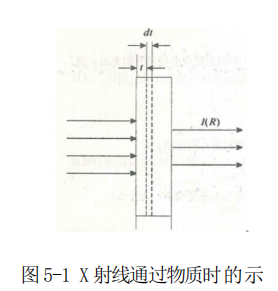
\includegraphics[scale=0.6]{t51}\end{center}
	如图 5-1 所示,设一厚度及成份均匀的吸收体,其厚度为 R,每立方厘米有N 个原子。若能量为 h ν的准直光 z 束,单位时间内垂直入射到吸收体单位面积上的光子数为 I0,那么通过厚度为 t 的物质后,透射出去的光子数为 I (t)并表示为:
	\begin{equation}
	I(t)=I_0e^{- \mu t}\label{11}
	\end{equation}
	其中,µ为该物质对某一能量 X 射线的线性吸收系数,$\mu = N \cdot \sigma $,$\sigma$为截面,其单位为 $cm^{2}/atom$,$\mu$的量纲为 $cm^{-1}$。对于原子序数为 Z 的原子,K 层的光电截面为$\sigma_{ph}(cm^{2}/atom)$。
	\begin{equation}
	\sigma_{ph}=\varphi_0 Z^5 \alpha^4 2^{5/2} \cdot (m_0c^2/hv)^{7/2}\label{sikao}
	\end{equation}

	其中$\varphi_0 = \frac{8}{3}\pi r_0^2$,$r_0 = e^2/m_0c^2$,$a = 2\pi e^2/hc \sim \frac{1}{137.04}$。

	对于汤姆逊散射,每个电子的截面是$\sigma_T(cm^2/electron)$,
	\begin{equation}
	\sigma_r = \frac{8\pi}{3}(\frac{e^2}{m_0c^2})^2 = 0.6653 \times 10^{-24}(cm^2/electron)
	\end{equation}
	\begin{equation}
	\mu_{ph} = N\sigma_{ph}
	\end{equation}
	\begin{equation}
	\mu_{T} = NZ\sigma_{T}
	\end{equation}
	总的线性吸收系数$\mu$为两者之和,即
	\begin{equation}
	\mu = \mu_{ph} + \mu_{T}
	\end{equation}
	质量吸收系数为$\mu_{m}$
	\begin{equation}
	\mu_m = \frac{\mu}{\rho}(cm^2/g) = \sigma \frac{N_A}{A}\label{77}
	\end{equation}
	所以\eqref{11}式又可表示为
	\begin{equation}
	I=I_0 e^{-\mu_m \rho t}\label{88}
	\end{equation}
	\begin{center}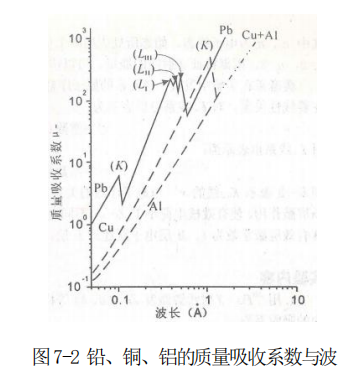
\includegraphics[scale=0.5]{t72}\end{center}

	\eqref{77}式中$ N_A$ 是阿佛加德罗常数,A 是原子量。图 5-2 表示了金属铅、铜、铝的质量吸收系数随波长的变化。在能量低于 0.1MeV 时,随着能量减小截面显示出尖锐的突变。实验表明,吸收系数突然下降的波长(吸收限)与 K 系激发限的波长很接近。在长波长区还有 L 突变与 M 突变存在,由于 L 层和 M 层构造的复杂性,这些突变不如 K 突变那样明显,并且有几个最大值。

	各种元素对不同波长入射 X 射线的吸收系数,由实验确定。元素的质量吸收系数与入射 X 射线能量之间的关系,可以用经验公式表示:
	
	对$E^{\prime} \textgreater E \textgreater E_k$
	\begin{equation}
	\begin{aligned}
	\mu_m=C^{\prime}_K \lambda^n(cm^2/g)\\ 
	\mu_m=C^{\prime}_K(12.3981/E)^n
	\end{aligned}
	\end{equation}
	对铝吸收体,$ E^{\prime}$为 6.20keV,$E_K$为 1.5596keV,$C^{\prime}_K $为 16.16,n 为 2.7345。

	\subsection{X 射线的特征谱}
	原子可以通过核衰变过程转换及轨道电子俘获,也可以通过外部射线如 X 射线,β射线(电子束)、$\alpha$粒子或其他带电粒子与原子中电子相互作用产生内层电子空位,在电子跃迁时产生特征 X 射线。玻耳理论指出电子跃迁时放出的光子具有一定的波长λ,它的能量为:
	\begin{equation}
	hv=Z^2 \frac{2\pi^2m_0e^4}{h^2}(\frac{1}{n_1^2}-\frac{1}{n_1^2})
	\end{equation}
	\begin{equation}
	hv={aZ}^2 \frac{m_0c^2}{2}(\frac{1}{n_1^2}-\frac{1}{n_1^2})
	\end{equation}
	其中 n1, n2 为电子终态、始态所处壳层的主量子数,对 Kα线系,n1=1, n2=2,对La线系,n1=2,n2=3,根据特征 X 射线的能量,可以辨认激发原子的原子序数。

	莫塞莱在实验中发现,轻元素的原子序数与$K_{\alpha}$及$L_{\alpha}$系特征X射线的频率 $v^{1/2}$之间存在线性关系。$K_{\alpha}$系的关系为:
	\begin{equation}
	v^{1/2}=k(Z-1)
	\end{equation}

	$L_{\alpha}$线系的关系表示为:
	\begin{equation}
	v^{1/2}=k(Z-7.4)\label{zuihou}
	\end{equation}

	\section{实验结果}
	\subsection{不同能量的X射线在铝中的吸收系数}
	查得对应元素密度如下表所示
	$$\begin{tabular}{|c|c|c|c|c|c|c|}
	\hline
	元素 & Ti & Cr & Fe & Cu & Zn & Ge   \\ \hline
	密度$(g/cm^3)$ & 4.51 & 7.20 & 7.87 & 8.96 & 7.14 & 6.24  \\ \hline
	\end{tabular}$$

	Ti、Cr、Fe、Cu、Zn、Ge金属膜样品的特征 X 射线强度随片数变化如下表所示
	$$\begin{tabular}{|c|c|c|c|c|c|c|c|c|}
	\hline
	膜片数 & 0 & 1 & 2 & 3 & 4 & 5 & 6 & 7   \\ \hline
	Ti每秒计数 & 9389 & 4695 & 2365 & 1180 & 604 & 303 & 152 & 76\\ \hline
	Cr每秒计数 & 9515 & 6213 & 4019 & 2635 & 1771 & 1153 & 768 & 496\\ \hline
	Fe每秒计数 & 9592 & 7338 & 5605 & 4349 & 3326 & 2523 & 1997 & 1518\\ \hline
	Cu每秒计数 & 9455 & 8176 & 7076 & 6154 & 5249 & 4639 & 4042 & 3424\\ \hline
	Zn每秒计数 & 9320 & 8383 & 7512 & 6601 & 5870 & 5307 & 4754 & 4184\\ \hline
	Ge每秒计数 & 9237 & 8557 & 7950 & 7409 & 6616 & 6323 & 5846 & 5408\\ \hline
	\end{tabular}$$
	
	易知,对固定的X射线,光强比等于粒子数比,故可用粒子数进行拟合。考虑到式\eqref{88}是一个指数函数,取对数有
	\begin{equation}
	ln({I_0})-ln(I)=-\mu_m \rho t
	\end{equation}
	
	其中,Ge的四片薄膜数据误差较大,我们绘图时去除。做拟合曲线如下
	\begin{figure}[H]
	\subfigure{
	\begin{minipage}{0.5\linewidth}
	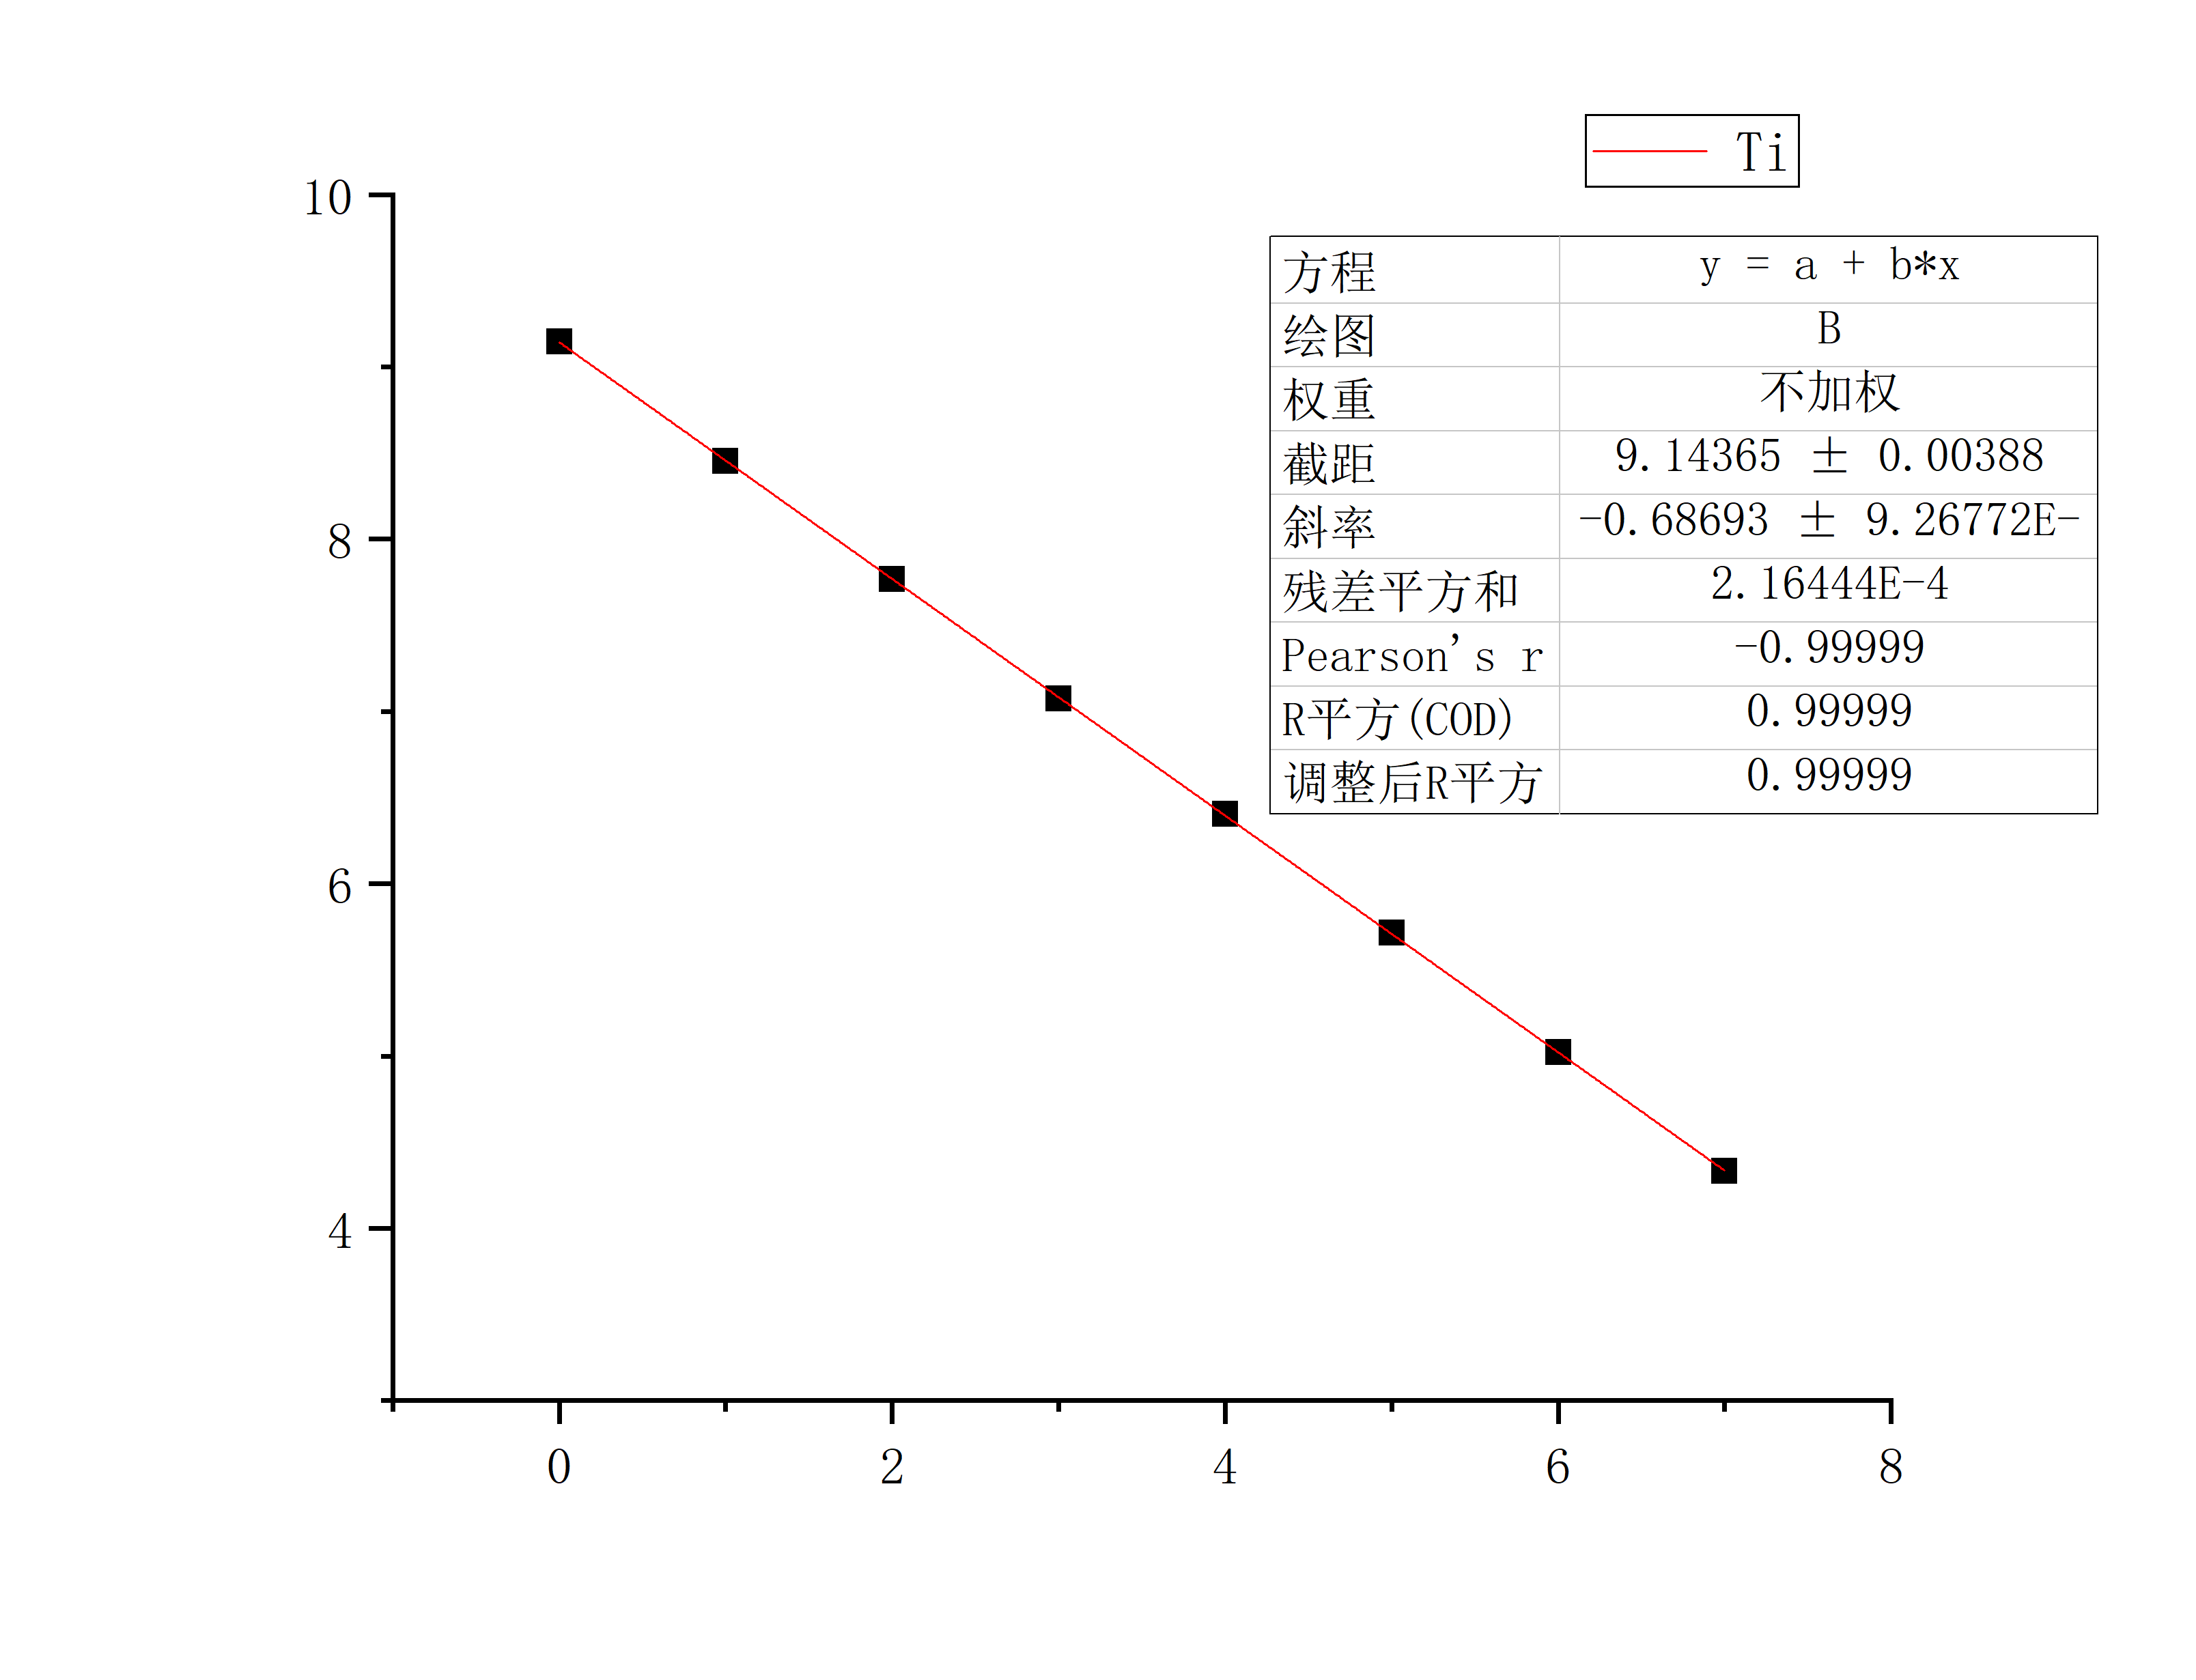
\includegraphics[scale=0.3]{t11}
	\end{minipage}
	}
	\subfigure{
	\begin{minipage}{0.25\linewidth}
	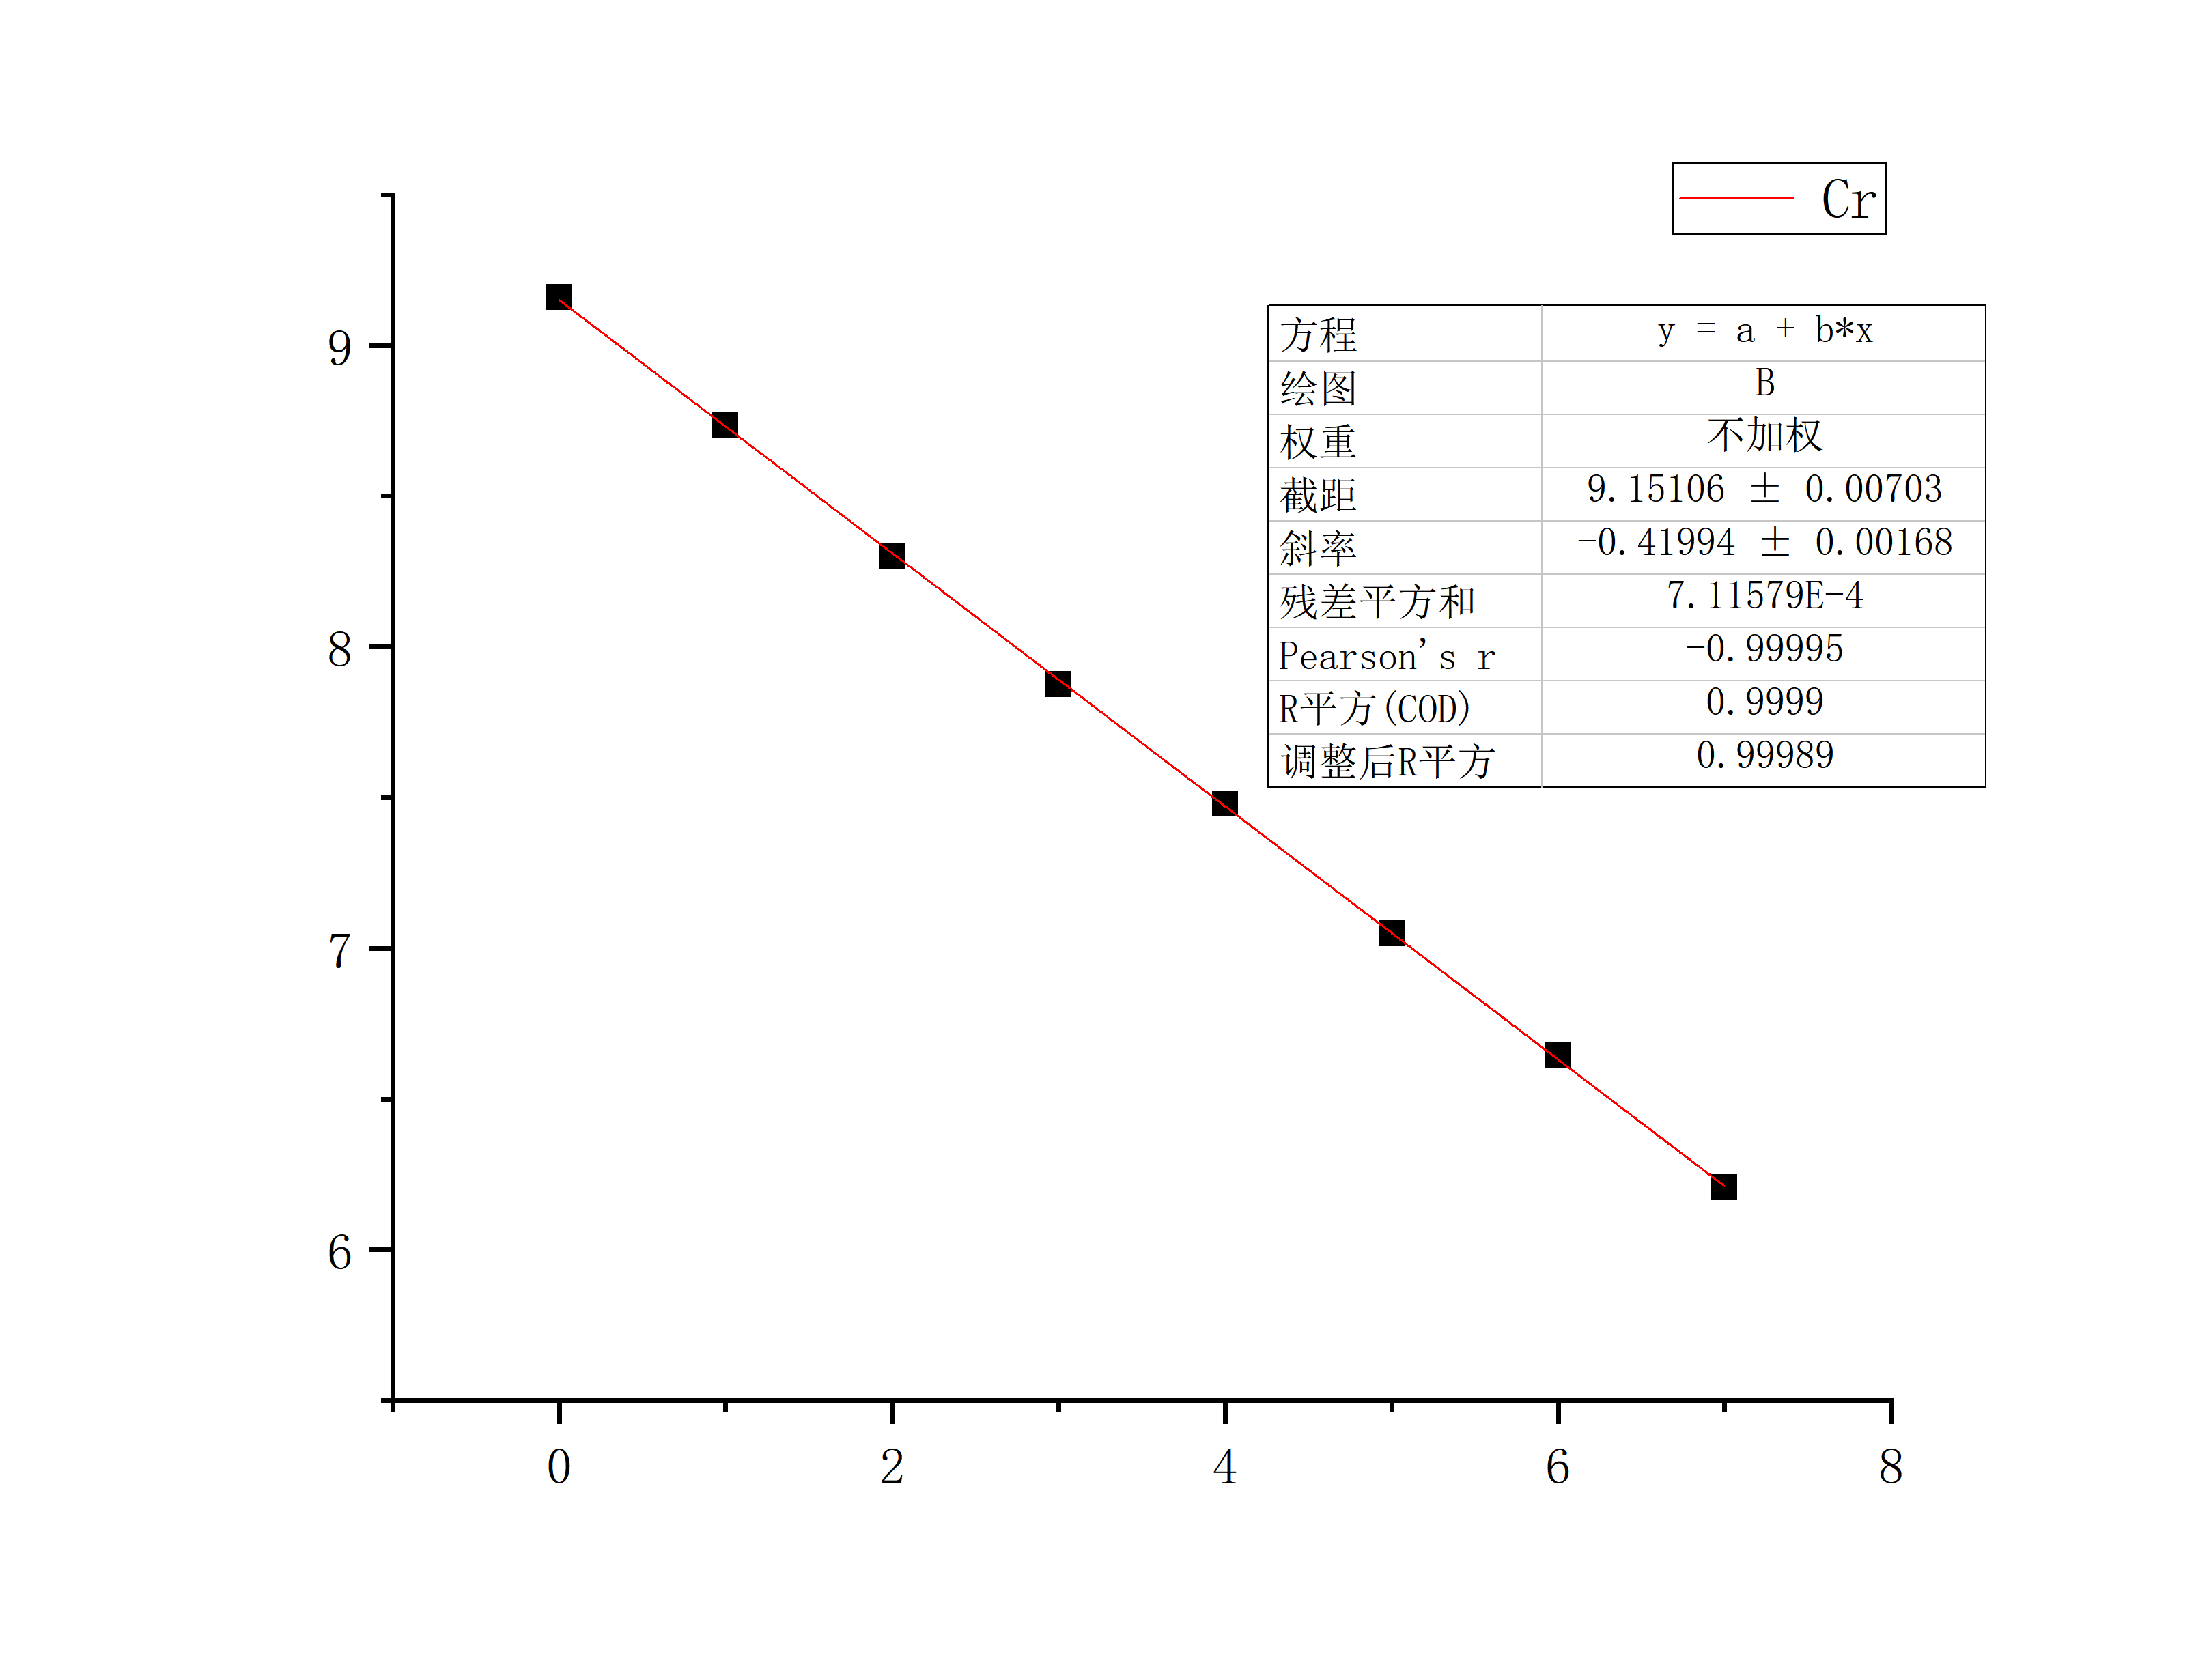
\includegraphics[scale=0.3]{t12}
	\end{minipage}
	}
	\end{figure}

	\begin{figure}[H]
	\subfigure{
	\begin{minipage}{0.5\linewidth}
	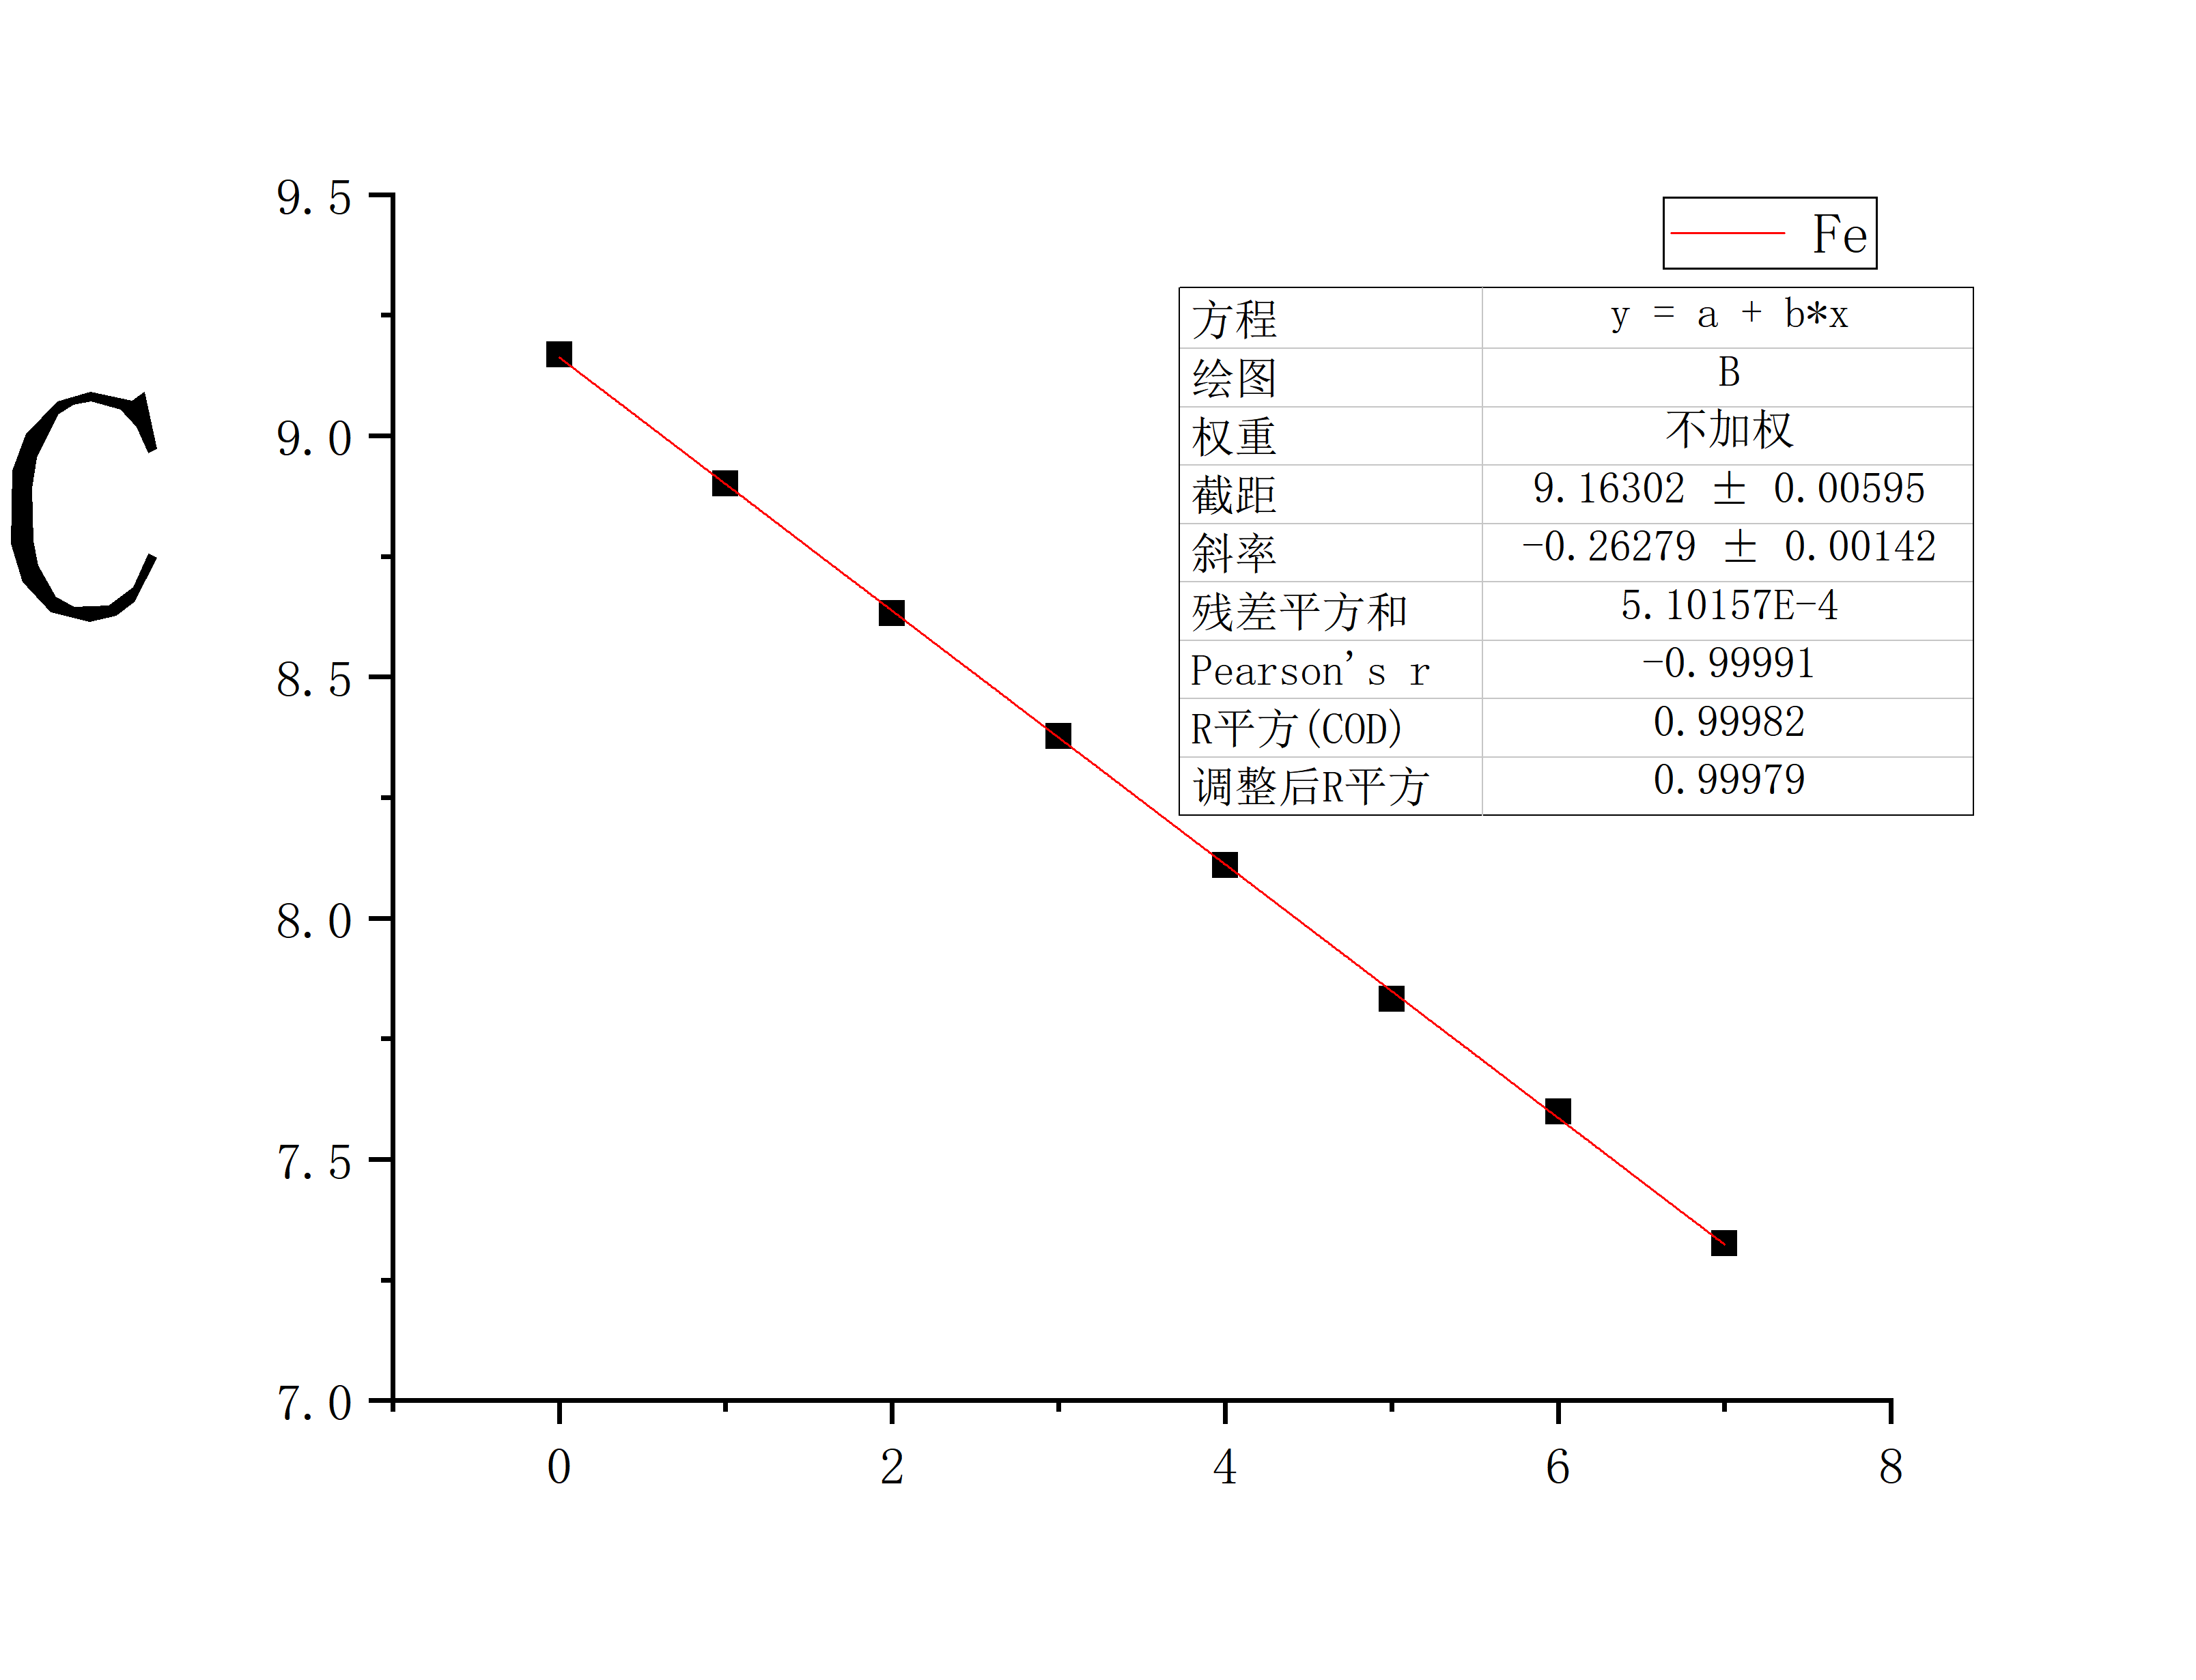
\includegraphics[scale=0.3]{t13}
	\end{minipage}
	}
	\subfigure{
	\begin{minipage}{0.25\linewidth}
	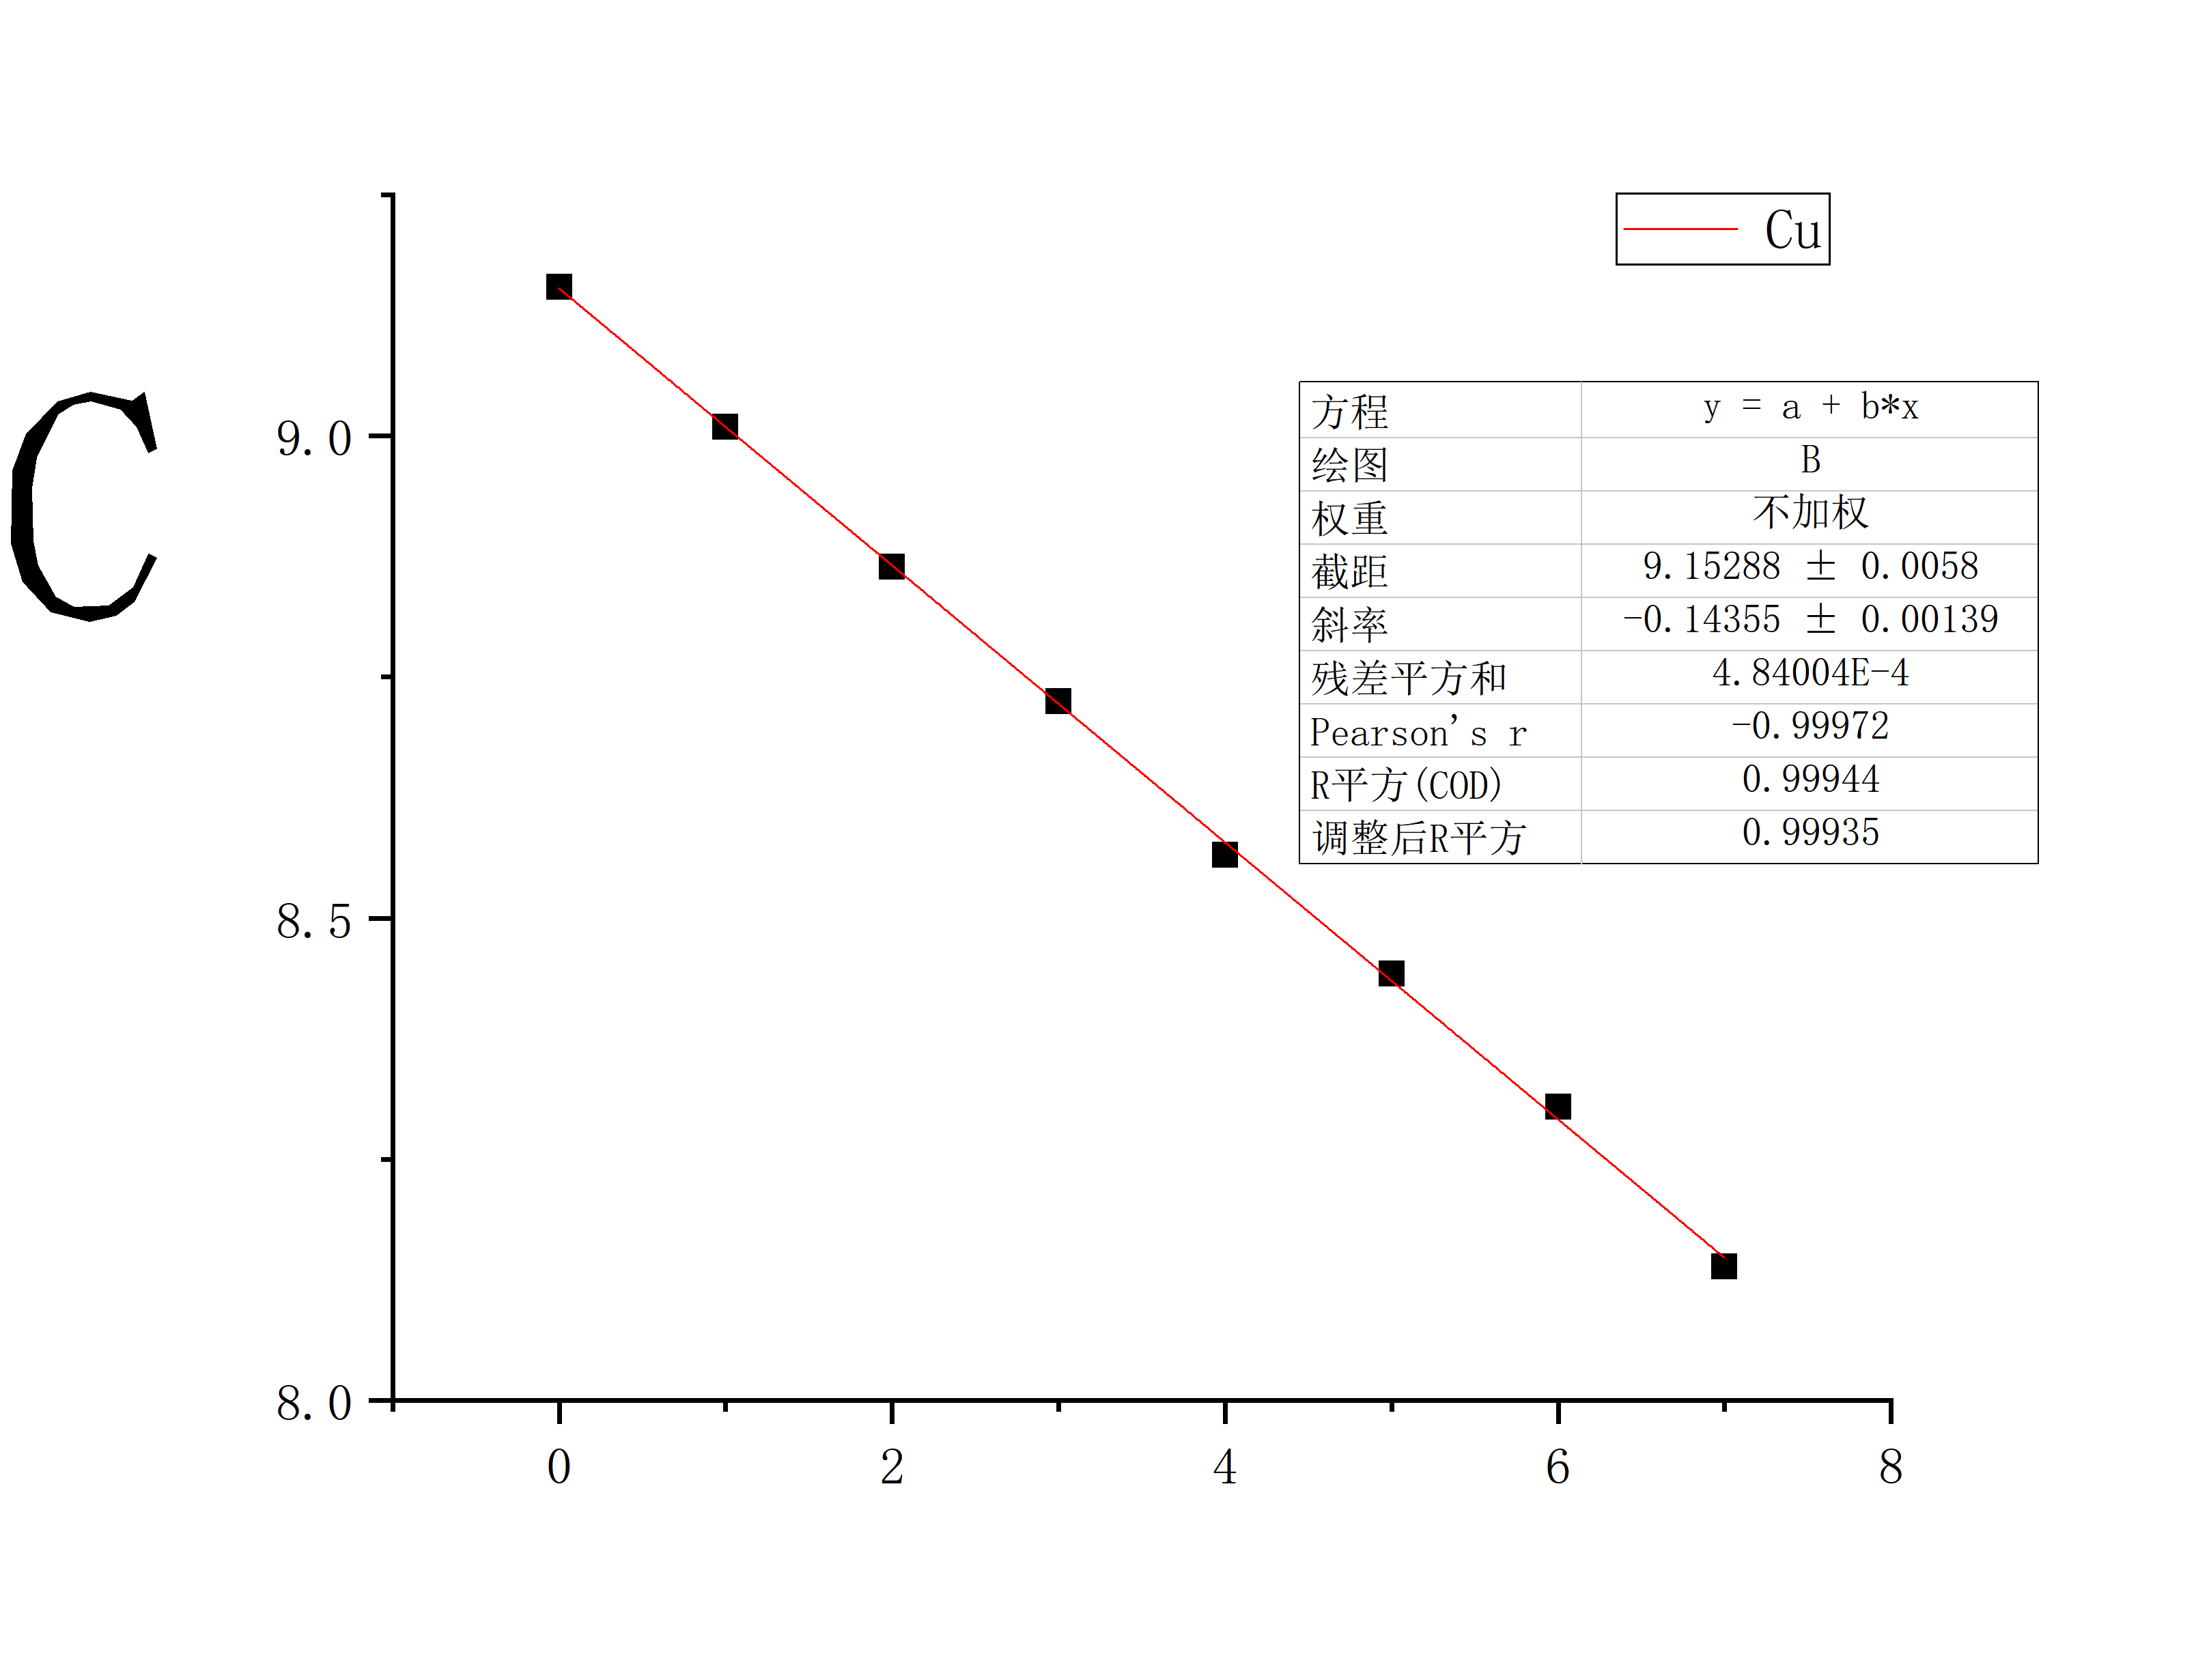
\includegraphics[scale=0.3]{t14}
	\end{minipage}
	}
	\end{figure}

	\begin{figure}[H]
	\begin{minipage}{0.5\linewidth}
	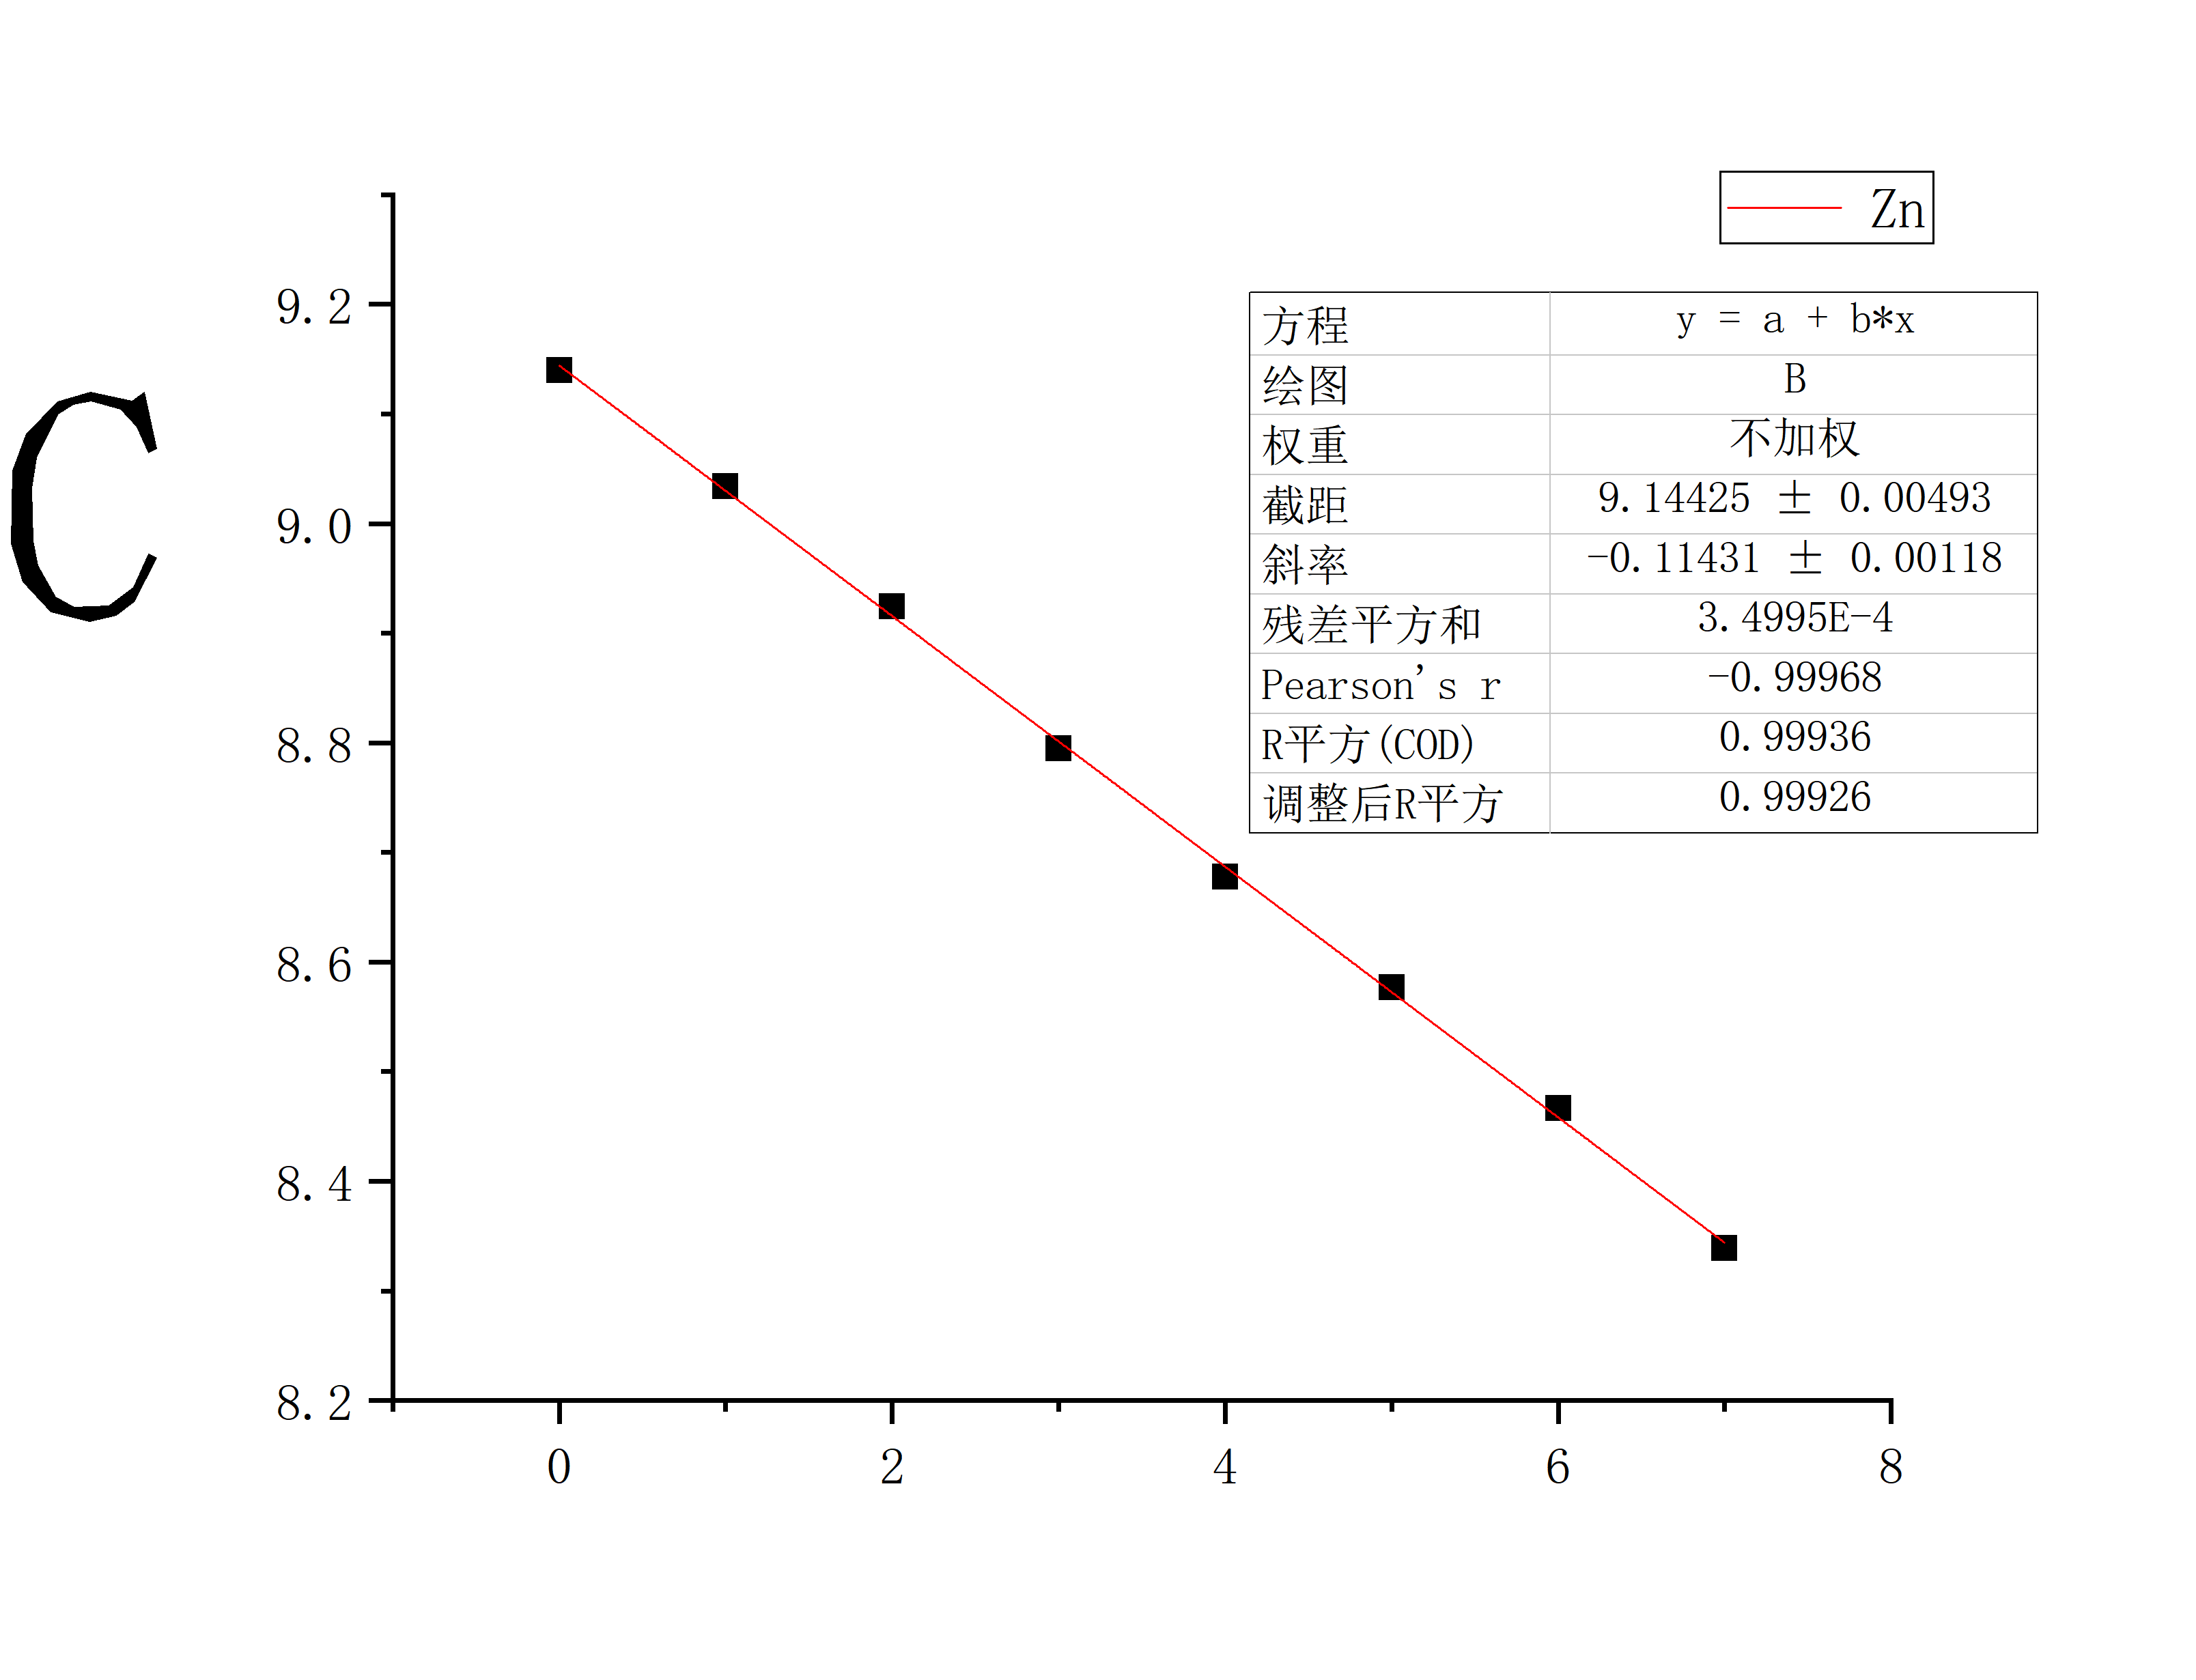
\includegraphics[scale=0.3]{t15}
	\end{minipage}
	\begin{minipage}{0.25\linewidth}
	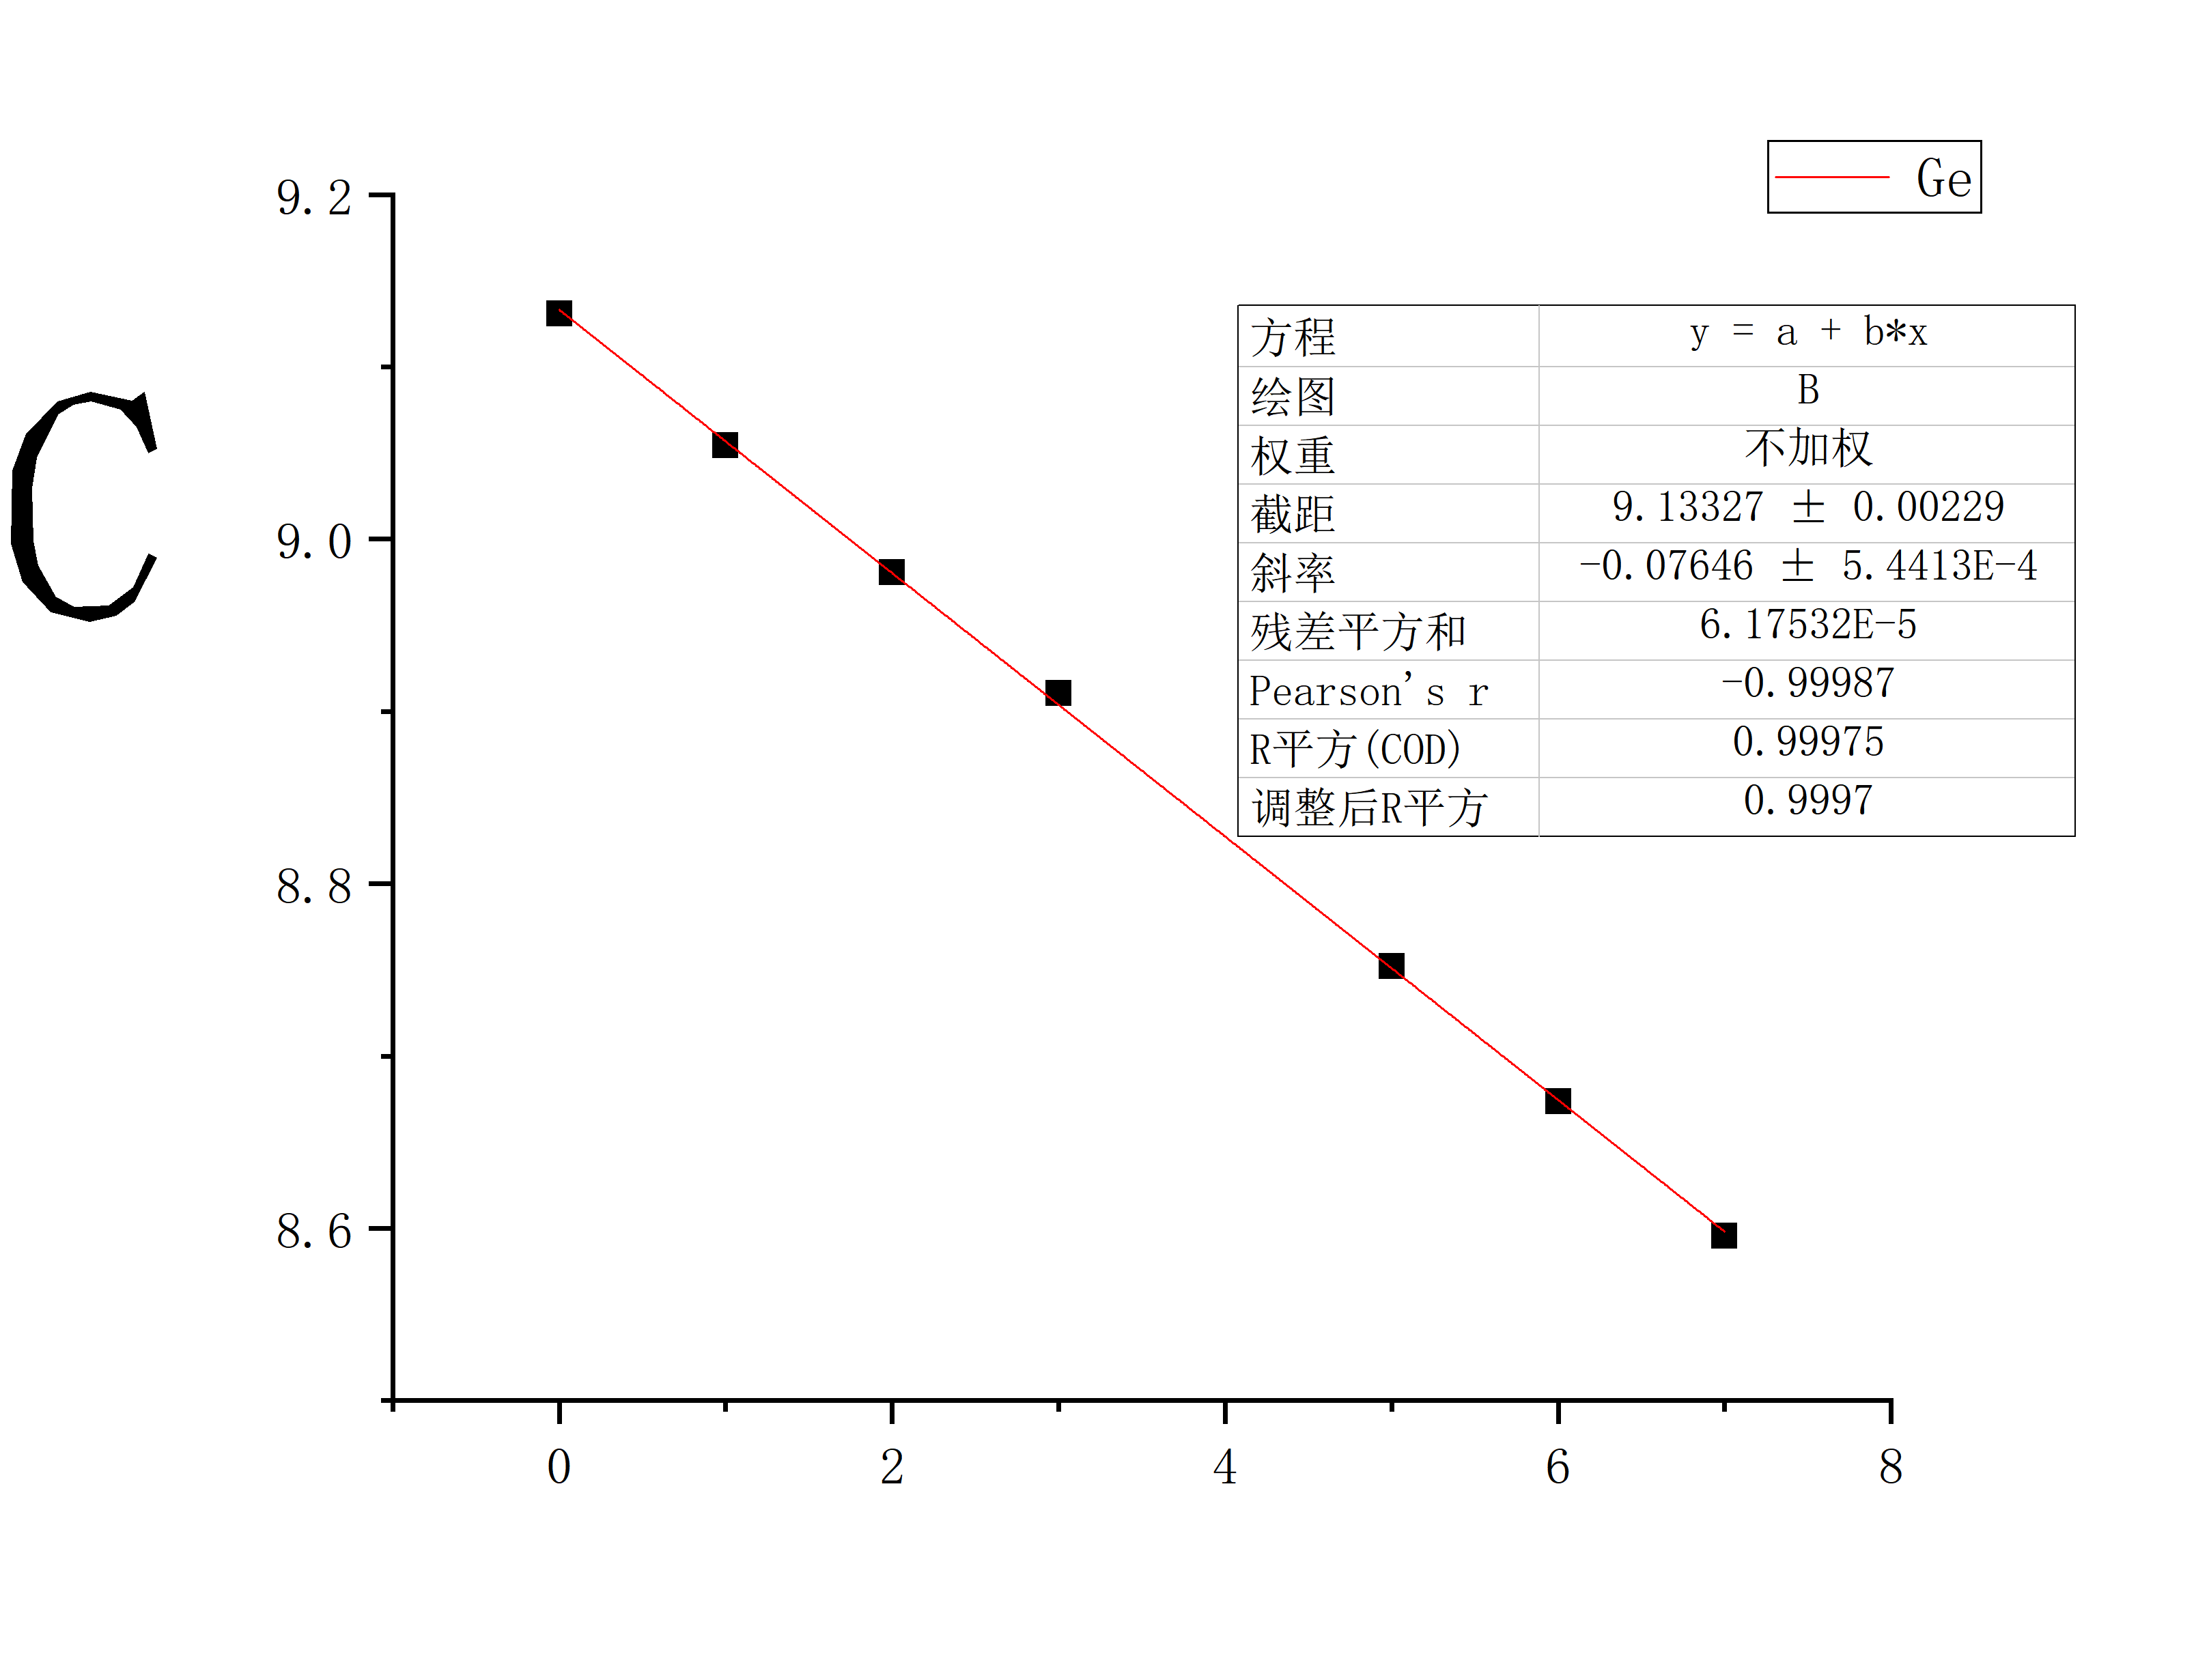
\includegraphics[scale=0.3]{t16}
	\end{minipage}
	\end{figure}

	考虑到单片薄膜10$\mu m$,利用表中的密度求得$\mu_m$如下
	$$\begin{tabular}{|c|c|c|c|c|c|c|}
	\hline
	元素 & Ti & Cr & Fe & Cu & Zn & Ge   \\ \hline
	$\mu_m(cm^2/g)$ & 152.3 & 58.3 & 33.4 & 16.0 & 16.0 & 12.2  \\ \hline
	\end{tabular}$$

	\subsection{不同元素的特征X射线谱}
	Ti、Cr、Fe、Cu、Zn、Ge的X射线峰位如下表
	$$\begin{tabular}{|c|c|c|c|c|c|c|}
	\hline
	元素 & Ti & Cr & Fe & Cu & Zn & Ge   \\ \hline
	峰位 & 2755 & 3287 & 3925 & 4860 & 5169 & 6002  \\ \hline
	$K\alpha$ & 4.51 & 5.41 & 6.4 & 8.04 & 8.63 & 9.24  \\ \hline
	\end{tabular}$$
	
	刻度如下图所示
	\begin{center}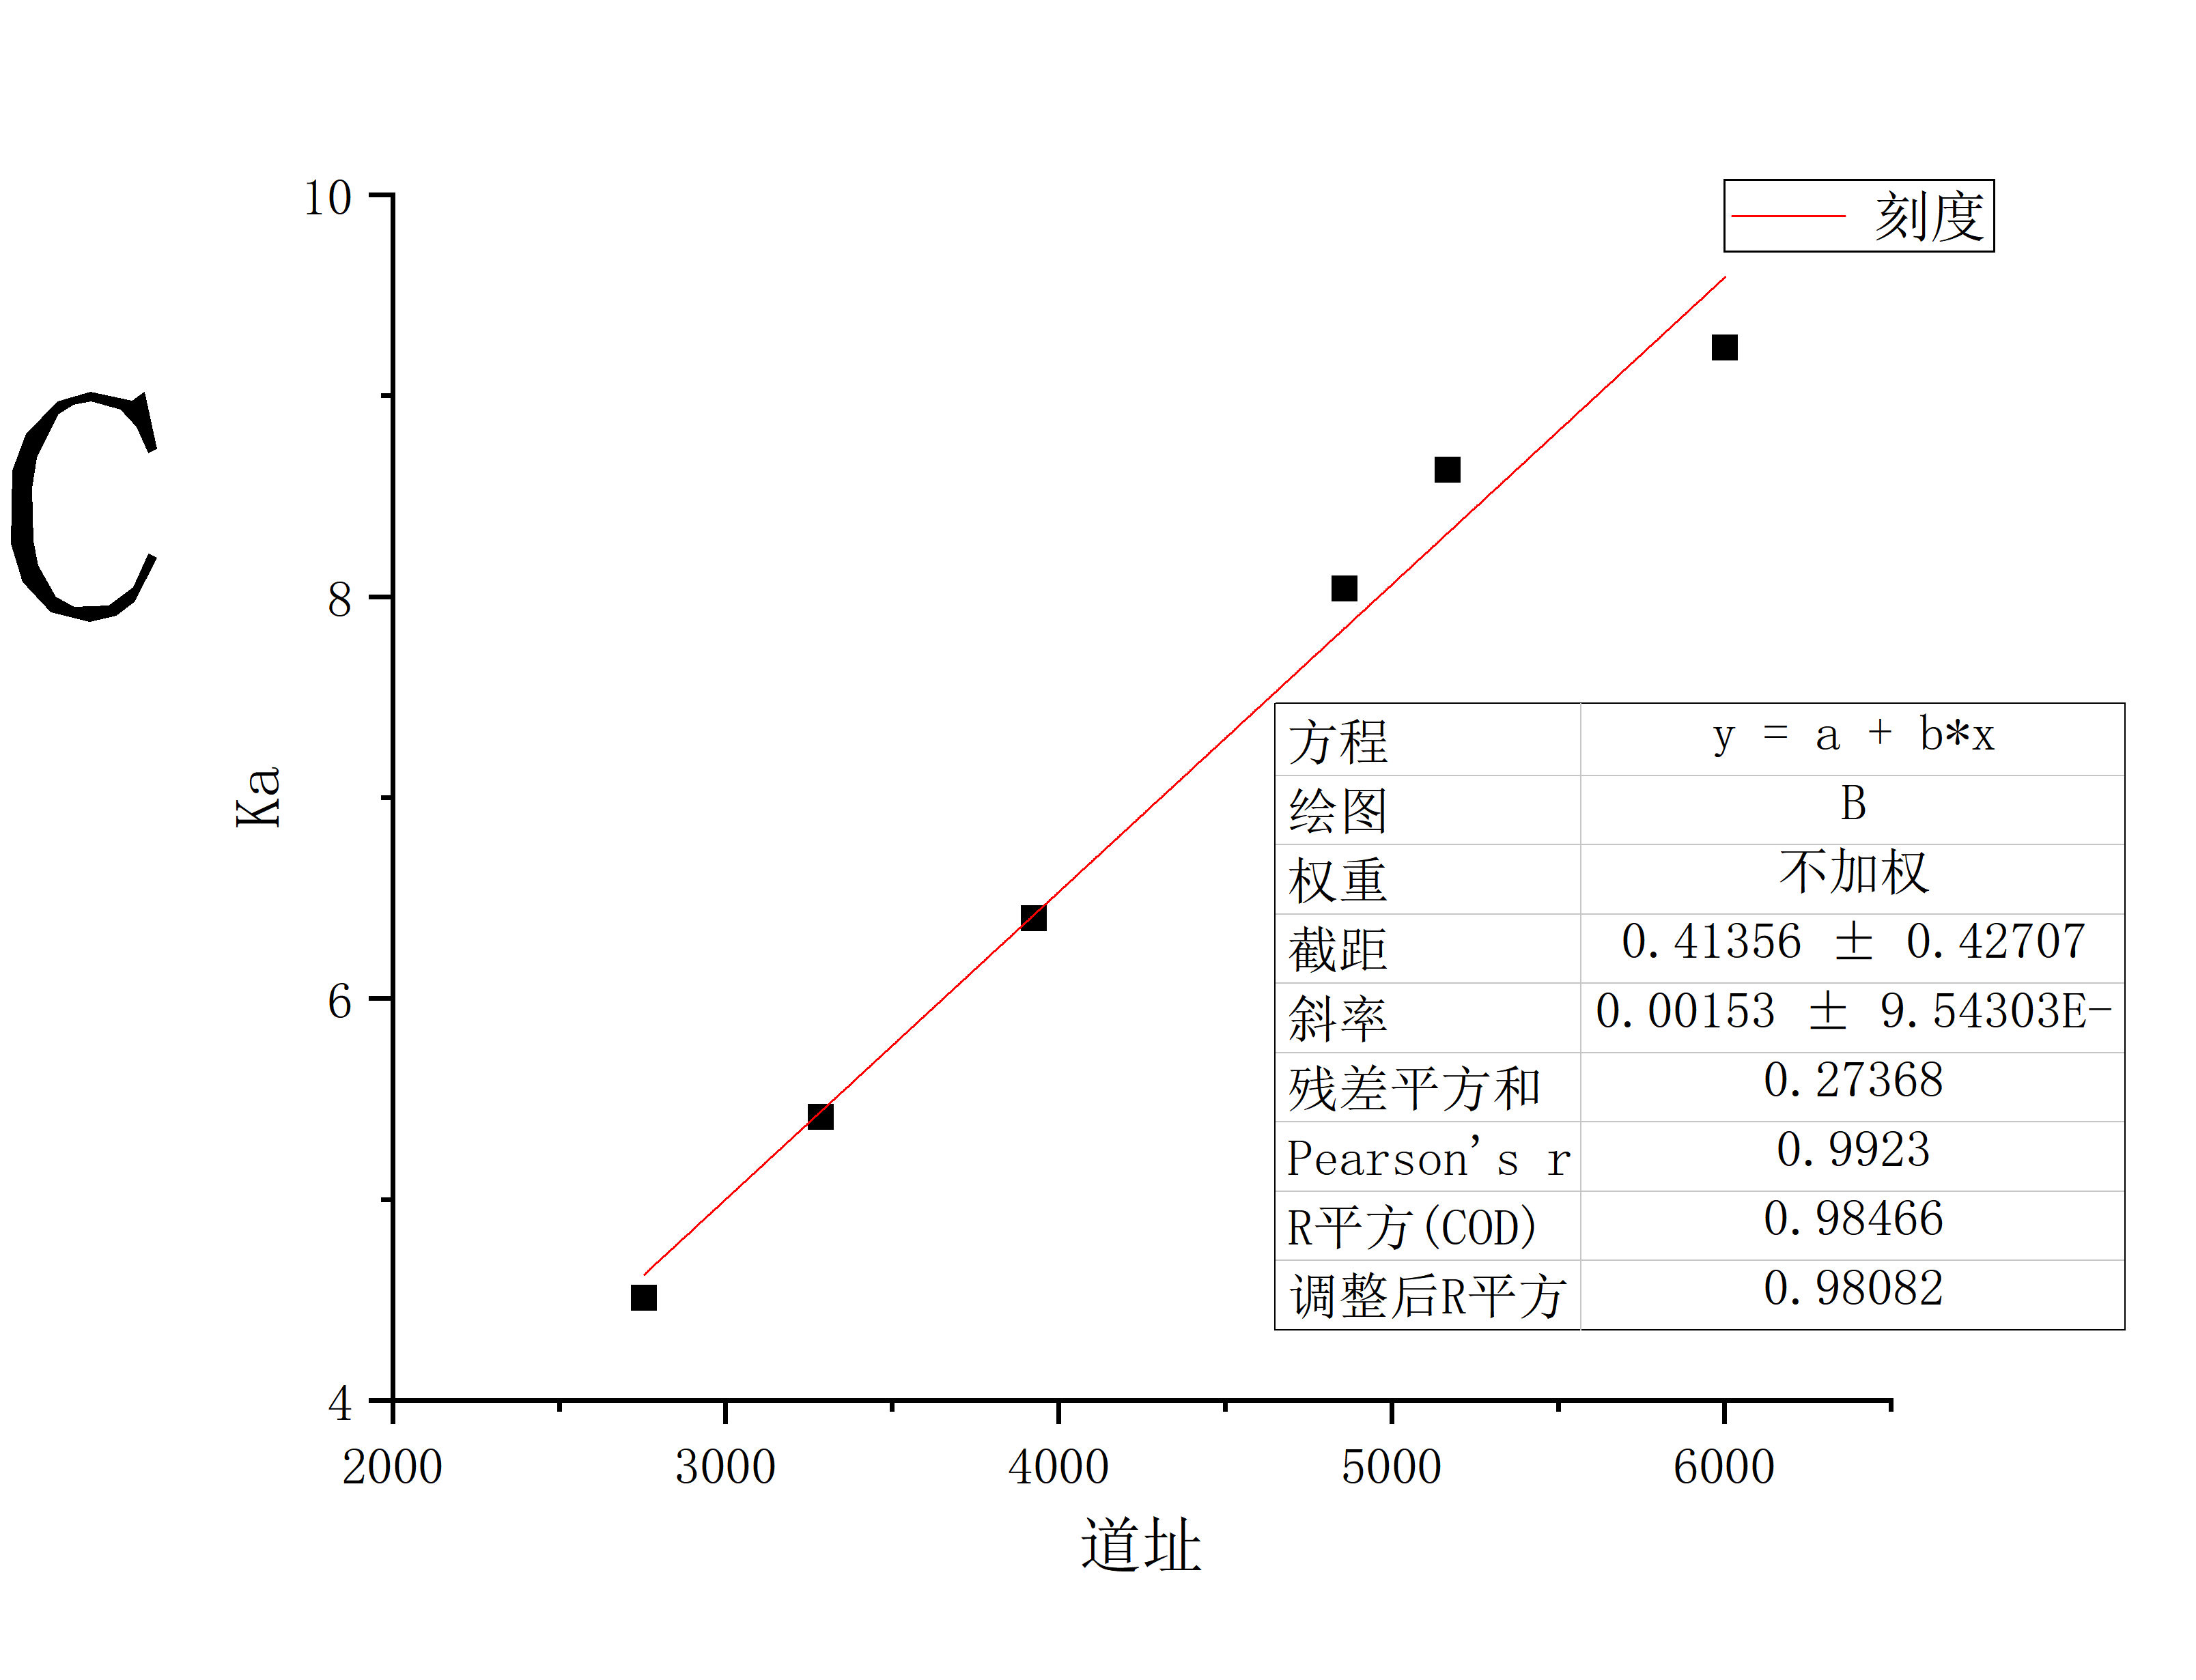
\includegraphics[scale=0.3]{t21}\end{center}

	结合三个未知元素的峰位分别为2970 ,4245 ,4607 。代入刻度公式
	\begin{equation}
	y=0.00153x+0.41356
	\end{equation}

	求得$K_{\alpha}$分别为4.96 ,6.91 ,7.46 。可知三个元素分别为V,Co,Ni。

	\subsection{$K_{\alpha}$射线拟合}
	九个元素如下
	$$\begin{tabular}{|c|c|c|c|c|c|c|c|c|c|}
	\hline
	元素 & Ti & Cr & Fe & Cu & Zn & Ge  & V & Co & Ni \\ \hline
	$(h \nu)^{1/2}$ & 2.124 & 2.326 & 2.530 & 2.835 & 2.938 & 3.040 & 2.227 & 2.623 & 2.731  \\ \hline
	\end{tabular}$$
	
	按最小二乘法作直线拟合如下
	\begin{center}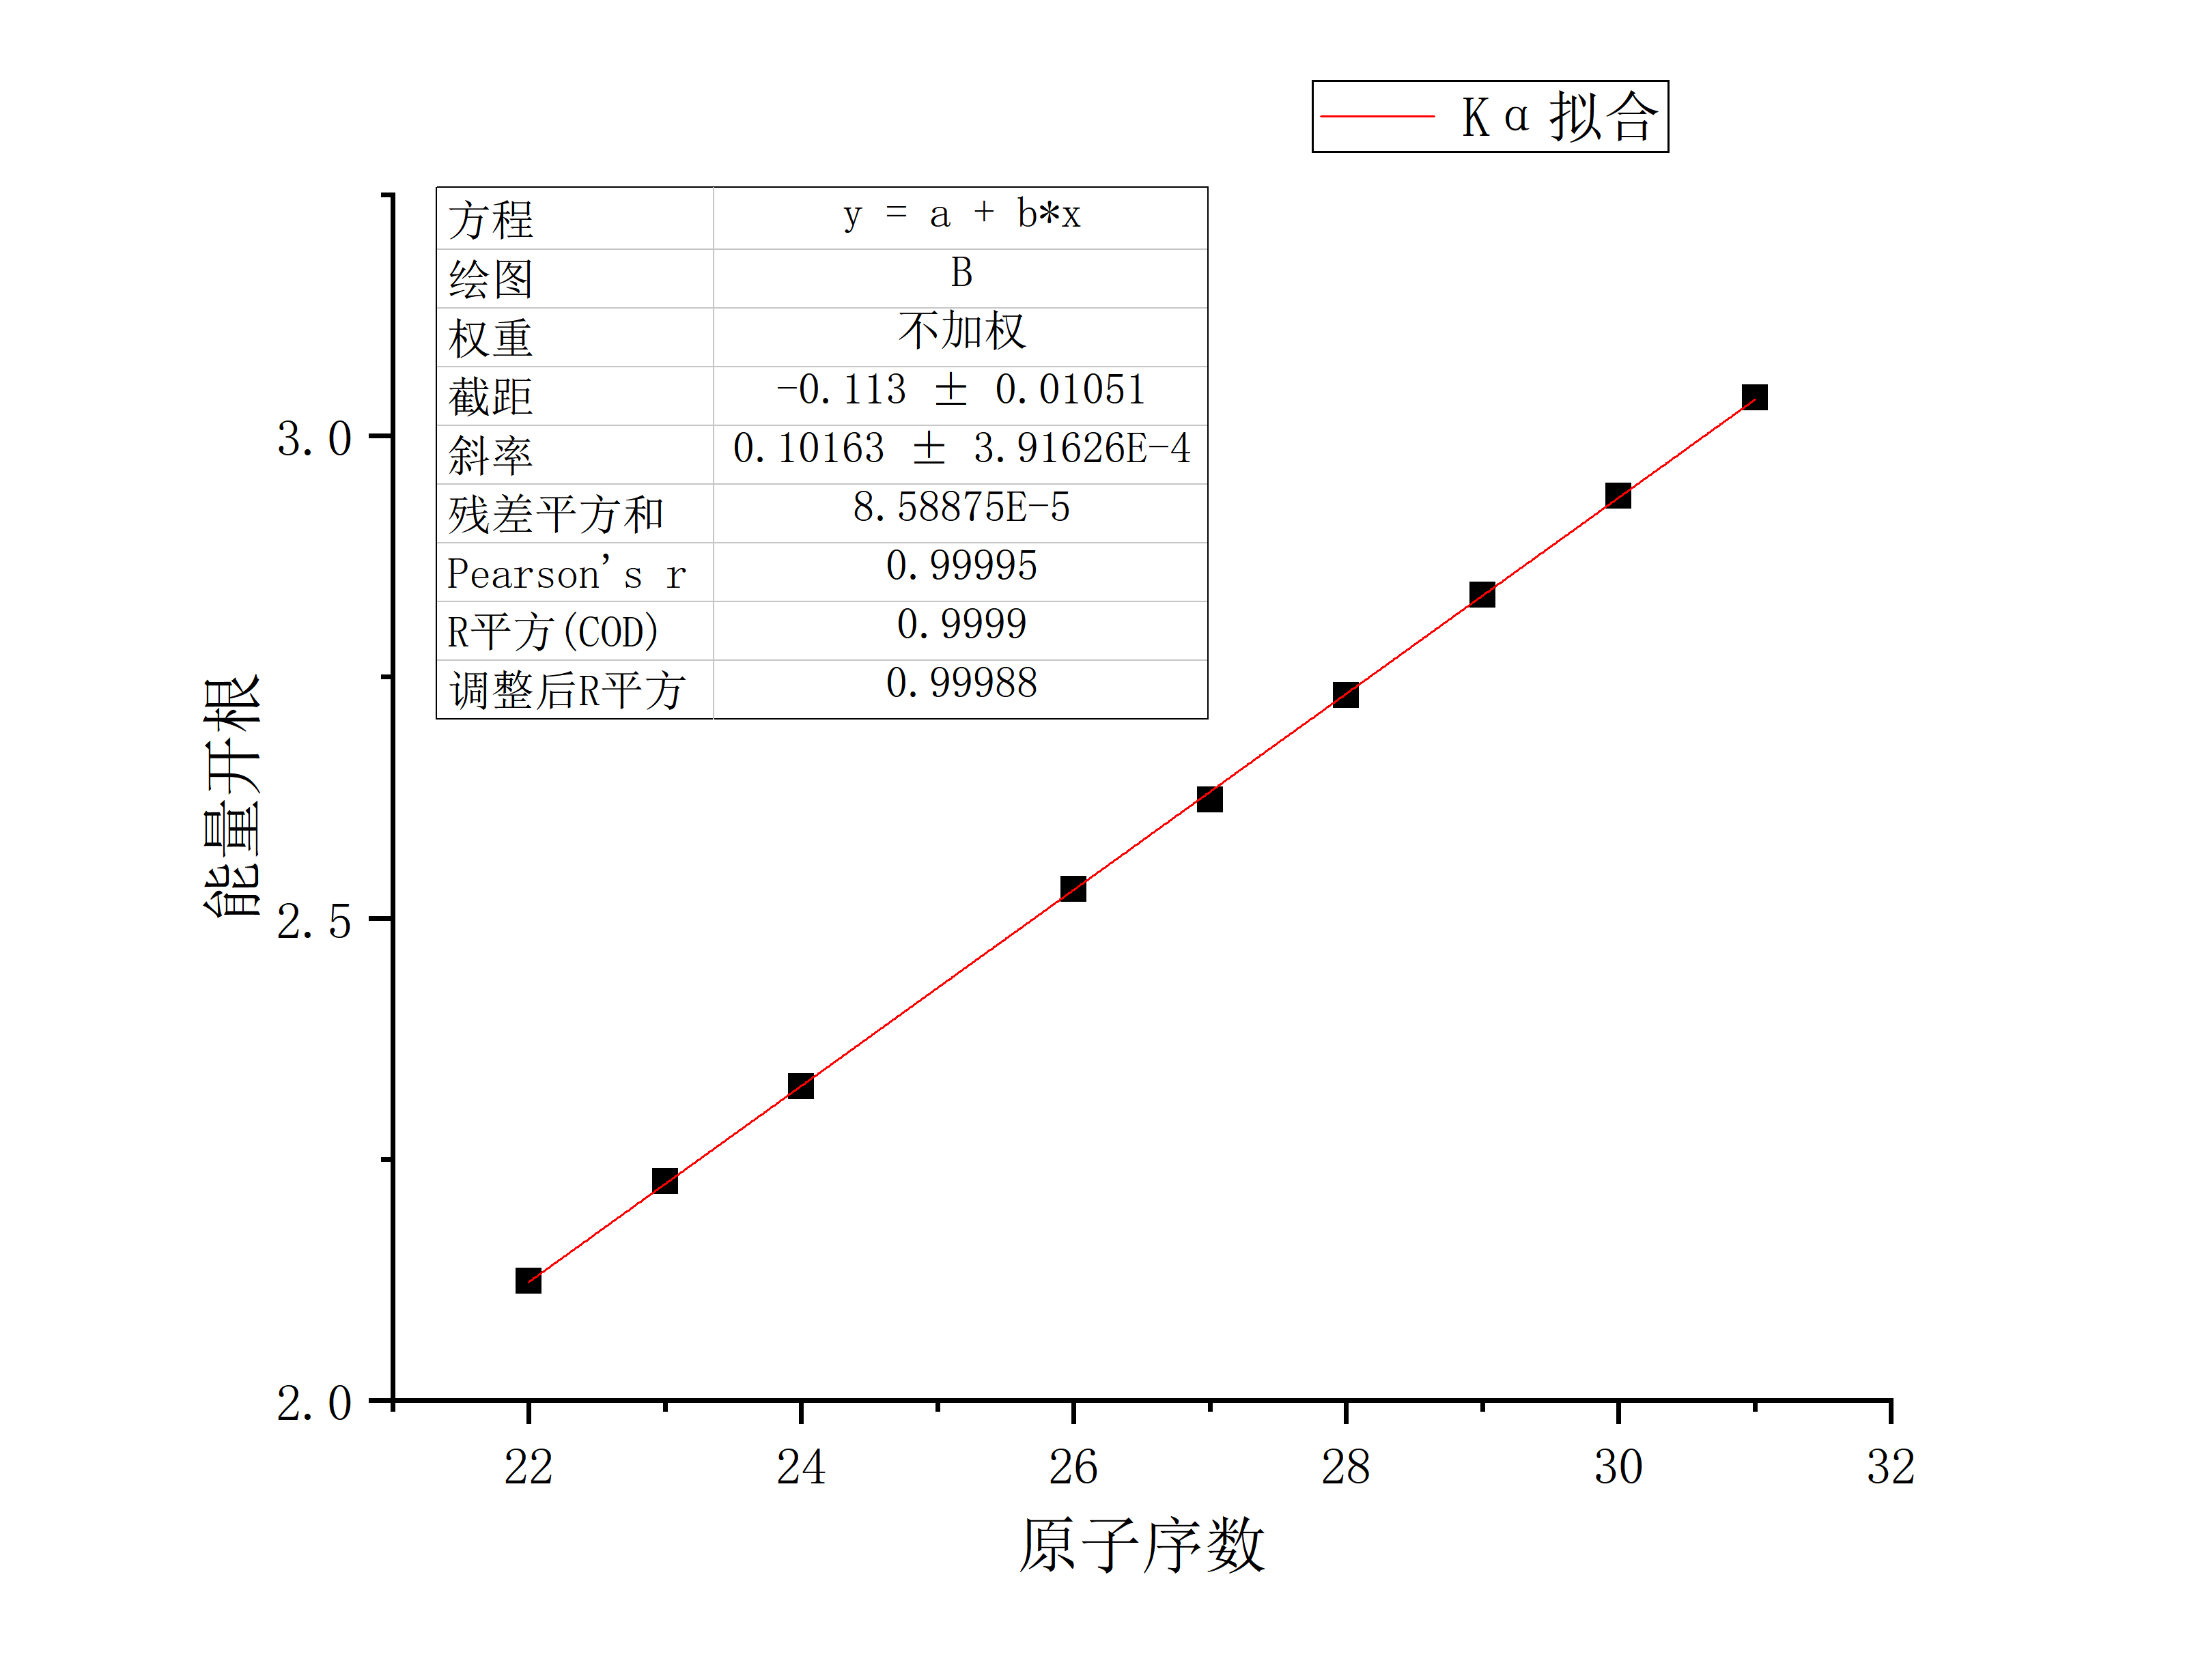
\includegraphics[scale=0.3]{t31}\end{center}

	可以看出$c^{\prime} = 0.1016$,$d=-1.112$。能量采取eV作单位后,斜率扩张微$10\sqrt{10}$倍, $c=3.213$ 。与式\eqref{zuihou}比较,发现吻合地还不错。



	\section{讨论}
	利用我们求出的$K_{\alpha}$射线拟合公式$(h \nu)^{1/2}=0.1016(Z-1.112)$,可以求得Ag的$K_{\alpha}$射线的能量为21.74keV,大于$^{238}Pu$源的 ULX 射线最大能量,所以应该是不可以激发的。

	对于汤姆逊散射,每个电子的截面是$\sigma_T = 0.6653 \times 10^{-24}(cm^2/electron)$。
	利用式\eqref{sikao},取铝的X射线能量1.49keV,可得铝原子 K 层的光电截面为 $ 2.98 \times 10^{-18}(cm^2/electron)=2.98 Mb$。铝原子光电截面远大于汤姆逊散射截面,所以本实验中汤姆逊散射截面不重要。

	当光线以$\theta$角斜射入金属膜(厚度为t)时,光线穿过$\frac{t}{sin\theta}$距离。即有
	$$ \frac{t}{cos\theta} \mu = t \mu^{\prime} $$
	其中,$\mu^{\prime}$为实验测得量,将略大于真实值。发散角为$10^{\circ}$时,真实值约为实验值的0.9848倍;发散角为$25^{\circ}$时,真实值约为实验值的0.9063倍;


%\end{multicols}
\end{document}